\documentclass{beamer}
\usepackage[french]{babel}
\usepackage{graphicx}
\usepackage{xcolor}
\usetheme{Luebeck}
\usecolortheme{seahorse}

\definecolor{darkgreen}{rgb}{0, 0.4, 0}
\definecolor{darkred}{rgb}{0.8, 0, 0}
\definecolor{darkblue}{rgb}{0, 0, 0.8}

\title{Projet n°8: Développez une application Web en utilisant Django}
\subtitle{OpenClassRooms - parcours python}
\author{Bérenger Ossété Gombé}

\begin{document}
\maketitle

\begin{frame}{Sommaire}
  \tableofcontents
\end{frame}

\section{Introduction}

\begin{frame}{Je me présente}
  \begin{block}{Bérenger Ossété Gombé}
    \begin{itemize}
    \item Bac Scientifique (2013).
    \item Maîtrise en informatique (2017).
    \item Reconversion web chez OpenClassRooms (janvier 2022).
    \end{itemize}
  \end{block}
\end{frame}

\begin{frame}{Contexte du projet}
  \begin{block}{Projet n°9, Parcours Python}
    \begin{itemize}
    \item Développer une application web en utilisant Django
    \item Utiliser le rendu côté serveur dans Django
    \end{itemize}
  \end{block}
\end{frame}

\begin{frame}{Contexte fictif}
  \begin{center}
    
\includegraphics[scale=0.2]{img/logo.png}
  \end{center}
  
  \begin{block}{LITReview}
    \begin{itemize}
    \item Équipe
      \begin{itemize}
      \item Alix, UX \textit{designer}.
      \item Sam, le directeur technique.
      \item Nous sommes \textit{lead} développeur Python.
      \end{itemize}
    \item Objectif: $\rightarrow$ Développement d'une application web.
    \end{itemize}    
  \end{block}
\end{frame}

\begin{frame}{L'application}
  \begin{block}{Deux types d'utilisateurs}
    \begin{itemize}
    \item Les utilisateurs qui \textbf{demandent des critiques} de documents.
    \item Les utilisateurs qui \textbf{recherchent des documents} guidés par les critiques.
    \end{itemize}
  \end{block}
\end{frame}

\section{Exigences}

\begin{frame}{Exigences fonctionnelles}
  \begin{block}{L'utilisateur peut:}
    \begin{itemize}
    \item Gérer son \textbf{compte} {\tiny(inscription, connexion, déconnexion)}.
    \item Consulter son \textbf{flux}.
    \item Créer un \textbf{ticket}.
    \item Publier une \textbf{critique} répondant ou non à un ticket.
    \item \textbf{Gérer} ses \textbf{tickets et critiques} {\tiny (consultation, édition, suppression)}
    \item \textbf{S'abonner} et se \textbf{désabonner} d'un utilisateur.
    \end{itemize}    
  \end{block}
\end{frame}

\section{Méthodes et Outils}

\begin{frame}{Outils logiciels}
  \begin{block}{Bibliothèques}
    \begin{itemize}
    \item Django (4.1)
    \item Django SASS (1.2.1)
    \item Pillow (9.2.0)
    \end{itemize}
  \end{block}
\end{frame}

\begin{frame}{Architecture du projet}
  \begin{block}{Découpage en applications}
    {\color{darkred}\textit{authentication}}, 
    {\color{darkblue}\textit{publication}}, 
    {\color{darkgreen}\textit{home}}
  \end{block}
  
  \begin{block}{Définition des principales urls}
    \tiny
    \begin{itemize}
    \item {\color{darkred} \url{login/}}
    \item {\color{darkred} \url{logout/}}
    \item {\color{darkred} \url{signup/}}
    \item {\color{darkblue} \url{tickets/}}
    \item {\color{darkblue} \url{tickets/<int:id>/edit}}
    \item {\color{darkblue} \url{tickets/<int:id>/review}}
    \item {\color{darkblue} \url{tickets/review}}
    \item {\color{darkblue} \url{reviews/<int:id>/edit}}

    \item {\color{darkgreen} \url{/}} (\textit{news feed})
    \item {\color{darkgreen} \url{social/}}
    \item {\color{darkgreen} \url{me/}}
    \end{itemize}
  \end{block}
\end{frame}

\begin{frame}[fragile]{Les modèles}
  \begin{block}{Utilisateur}
    \begin{lstlisting}
      class User(AbstractUser):
          pass
    \end{lstlisting}    
  \end{block}
\end{frame}

\begin{frame}[fragile]{Les modèles}
  \begin{block}{Les Tickets}
    \tiny
    \begin{lstlisting}
      class Ticket(models.Model):
          title = models.CharField(max_length=128)
          description = models.TextField(max_length=248,
          blank=True)
          user = models.ForeignKey(to=settings.AUTH_USER_MODEL,
          on_delete=models.CASCADE)
          image = models.ImageField(null=True, blank=True)
          time_created = models.DateTimeField(auto_now_add=True)
    \end{lstlisting}    
  \end{block}

  \begin{block}{Les Critiques}
    \tiny
    \begin{lstlisting}
      class Review(models.Model):
          ticket = models.ForeignKey(to=Ticket, on_delete=models.CASCADE)
          rating = models.PositiveSmallIntegerField(validators=[
            MinValueValidator(0),
            MaxValueValidator(5)
          ])
          user = models.ForeignKey(to=settings.AUTH_USER_MODEL,
          on_delete=models.CASCADE)
          headline = models.CharField(max_length=128)
          body = models.TextField(max_length=8192, blank=True)
          time_created = models.DateTimeField(auto_now_add=True)
    \end{lstlisting}
  \end{block}
\end{frame}

\begin{frame}[fragile]{Les modèles}
  \begin{block}{Les Abonnements}
    \tiny
    \begin{lstlisting}
      class UserFollows(models.Model):
          user = models.ForeignKey(to=settings.AUTH_USER_MODEL,
          on_delete=models.CASCADE,
          related_name='following')
          followed_user = models.ForeignKey(to=settings.AUTH_USER_MODEL,
          on_delete=models.CASCADE,
          related_name='followed_by')
          
          class Meta:
              unique_together = ('user', 'followed_user')
    \end{lstlisting}    
  \end{block}
\end{frame}

\begin{frame}[fragile]{Les contrôleurs}
  \begin{block}{Utilisation de vues génériques}
    \tiny
    \begin{lstlisting}
      class SignupPage(generic.CreateView):
          form_class = forms.UserForm
          success_url = reverse_lazy('login')
          template_name = 'authentication/signup.html'


      class LoginPage(LoginView):
          form_class = forms.LoginForm
          template_name = 'authentication/login.html'
          next_page = reverse_lazy('signup')


      class LogoutPage(LogoutView):
          next_page = reverse_lazy('login')

    \end{lstlisting}
  \end{block}
\end{frame}

\begin{frame}[fragile]{Les contrôleurs}
  \begin{block}{Utilisation de vues basées sur des classes}
    \tiny
    \begin{lstlisting}
      class CreateTicketReview(LoginRequiredMixin, View):
          def get(self, request, id):
              ticket = get_object_or_404(models.Ticket, id=id)
              author = User.objects.get(id=ticket.user_id)
              form = forms.ReviewForm()
              
              return render(request, 'publication/ticket_review.html', {
                'ticket': ticket,
                'author': author,
                'form': form
              })

          def post(self, request, id):
              ticket = get_object_or_404(models.Ticket, id=id)
              author = User.objects.get(id=ticket.user_id)
              form = forms.ReviewForm(request.POST)
              
              if form.is_valid():
                  review = form.save(commit=False)
                  review.ticket = ticket
                  review.user = request.user
                  review.save()
                  return redirect('me')
              
              return render(request, 'publication/ticket_review.html', {
                'ticket': ticket,
                'author': author,
                'form': form
              })
    \end{lstlisting}
  \end{block}
\end{frame}

\begin{frame}[fragile]{Les vues}
  \begin{block}{Vues partielles}
    \tiny
    \begin{center}
      \fbox{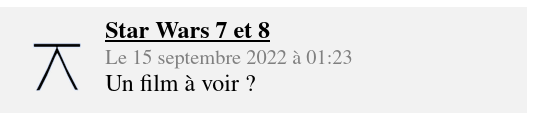
\includegraphics[scale=0.2]{img/ticket.png}}
      \fbox{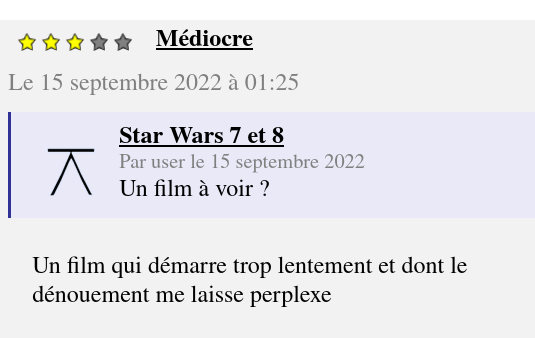
\includegraphics[scale=0.2]{img/review.png}}
    \end{center}

    \begin{lstlisting}
      
      
    \end{lstlisting}
  \end{block}
\end{frame}

\begin{frame}[fragile]{Les vues}
  \begin{block}{Vues héritées}
    \tiny
    \begin{lstlisting}{language=html}
      
      
          <!-- Code de la vue-->
      
    \end{lstlisting}
  \end{block}
\end{frame}

\section{Démonstration}

\section{Conclusion}


\end{document}
